% Provenance (never printed): see sources/outline_sources.md (Year 2: the solar nebula
% and the condensation sequence; planetesimals and embryos; chondrites, achondrites and
% irons; the age of the Solar System; differentiation of planets). Curves from
% figdata/bachelor-2/nebula.py, condensation.py, al26.py, meteorites.py; exercise and
% problem values in the Book 4 scratch calculator calc/ch02.py.
\chapter{Formation des planètes et météorites}\label{ch:b2:planet-formation-meteorites}

Chaque année, environ quinze mille tonnes de poussière venue de l'espace entrent dans
l'atmosphère terrestre~; la plupart brûlent ou retombent sous forme de sphérules
microscopiques, et de temps en temps une pierre de la taille d'un poing tombe avec une boule
de feu et un bang supersonique. La plupart de ces pierres sont des fragments d'astéroïdes, et
beaucoup n'ont guère changé depuis leur formation. Sciée puis polie, une pierre montre des
billes de roche jadis fondue, de l'ordre du millimètre, des grains blancs et irréguliers de
minéraux de calcium et d'aluminium, des paillettes de métal, le tout pris dans un ciment
sombre à grain fin. Les grains blancs sont les plus anciens solides du système solaire~: les
isotopes du plomb les datent de 4567~Ma. Un second chronomètre, la désintégration d'un
isotope radioactif de l'aluminium disparu depuis longtemps, date les autres composants par
rapport à eux, à une fraction de million d'années près. Ce chapitre suit le disque du
chapitre précédent lorsqu'il se transforme en planètes~: quels solides se condensent à partir
du gaz qui se refroidit, et où~; comment la poussière croît en corps de quelques kilomètres,
puis en planètes~; ce que sont les \omterm{def:b2:planet-formation-meteorites:fall-find}{météorites}, et comment elles datent ces événements~; et
pourquoi certains des premiers corps ont fondu et formé des noyaux de fer, tandis que
d'autres sont restés tels qu'ils s'étaient formés.
% ledger: rojas21:flux, lugaro:cai, gail:meteorites

\begin{recall}
Les jeunes étoiles sont entourées de \omterm{def:b2:ism-star-formation:disc}{disques protoplanétaires}, qui disparaissent en quelques
millions d'années~; un grain de poussière éclairé à la distance $r$ d'une étoile de luminosité
$L$ s'établit à $T = \bigl(L/(16\pi\sigma r^2)\bigr)^{1/4}$ (\cref{ch:b2:ism-star-formation}).
Les astéroïdes sont les petits corps rocheux ou métalliques du système solaire, dont la
plupart orbitent entre Mars et Jupiter (volume de première année). Un noyau radioactif se
désintègre, avec la probabilité $\lambda$ par unité de temps~: $N = N_0 e^{-\lambda t}$~; la
demi-vie vaut $\ln 2/\lambda$, et la durée de vie moyenne $\tau = 1/\lambda$ (les volumes de
physique). Dans un système fermé, des échantillons cogénétiques de rapports parent-fils
différents se placent sur une droite, l'isochrone, dont la pente donne l'âge et dont
l'ordonnée à l'origine donne le rapport initial (volume de première année). Élever la
température d'une masse $m$ de capacité thermique massique $c$ de $\Delta T$ demande l'énergie
$mc\,\Delta T$ (les volumes de physique).
\end{recall}

\section{La nébuleuse solaire}

\begin{definition}[Nébuleuse solaire]\label{def:b2:planet-formation-meteorites:nebula}
La \emph{nébuleuse solaire}\index{nébuleuse solaire} est le \omterm{def:b2:ism-star-formation:disc}{disque protoplanétaire} de gaz et
de poussière qui entourait le jeune Soleil et d'où sont issus les planètes, leurs
satellites, les astéroïdes et les comètes.
\end{definition}

Quelle masse contenait-elle~? Une limite inférieure vient des planètes elles-mêmes.
Ajoutons à chacune assez d'hydrogène et d'hélium pour lui donner la composition du
Soleil, répartissons le résultat sur un anneau centré sur son orbite~; la densité
surfacique, c'est-à-dire la masse par unité de surface du disque, décroît avec la
distance au Soleil. Cette reconstruction est la \emph{nébuleuse solaire de masse
minimale}\index{nébuleuse solaire de masse minimale}. Dans une version très utilisée, la
densité surfacique du gaz vaut
\[
  \Sigma_g = \qty{2200}{g.cm^{-2}}\left(\frac{r}{\qty{1}{au}}\right)^{-3/2},
\]
et celle des solides $\Sigma_p = \qty{33}{g.cm^{-2}}\,Z_{\mathrm{rel}}\,
(r/\qty{1}{au})^{-3/2}$, où $Z_{\mathrm{rel}}$ est la fraction de la matière
condensable réellement solide~: $0.33$ là où seuls la roche et le métal ont condensé,
environ $0.78$ là où la glace d'eau s'y est jointe, $1$ au-delà de l'endroit où le méthane gèle.
Les nombres sont incertains~: la teneur en éléments lourds de Jupiter n'est connue
qu'à un facteur quatre près, et les planètes ne se sont pas nécessairement formées
là où elles orbitent aujourd'hui.
% ledger: cy10:mmsn

\begin{proposition}[Masse d'un disque]\label{prop:b2:planet-formation-meteorites:disc-mass}
Un disque de densité surfacique $\Sigma(r) = \Sigma_1 (r/r_1)^{-3/2}$ contient, à
l'intérieur du rayon $R$, la masse
\[
  M(R) = 4\pi\Sigma_1 r_1^2 \left(\frac{R}{r_1}\right)^{1/2}.
\]
La plus grande part de la masse se trouve loin à l'extérieur~: doubler le rayon augmente la
masse de \qty{41}{\percent}.
\end{proposition}

\begin{proof}
Un anneau de rayon $r$ et de largeur $\mathrm dr$ a pour aire $2\pi r\,\mathrm dr$, donc
\[
  M(R) = \int_0^R 2\pi r\,\Sigma_1 \left(\frac{r}{r_1}\right)^{-3/2}\mathrm dr
       = 2\pi\Sigma_1 r_1^{3/2}\int_0^R r^{-1/2}\,\mathrm dr
       = 4\pi\Sigma_1 r_1^{3/2} R^{1/2},
\]
ce qui donne la formule~; l'intégrale converge en $r = 0$. Doubler $R$ multiplie
$M$ par $\sqrt 2 = 1.41$.
\end{proof}

Avec $\Sigma_1 = \qty{2.2e4}{kg.m^{-2}}$ à $r_1 = \qty{1}{au}$, la \omterm{def:b2:planet-formation-meteorites:nebula}{nébuleuse solaire} de masse minimale
contient $0.03$ masse solaire à l'intérieur de \qty{100}{au}
(\cref{exo:b2:planet-formation-meteorites:5}). Les disques observés autour d'étoiles âgées d'un million
d'années, pesés grâce à l'éclat millimétrique de leurs poussières, contiennent \numrange{0.001}{0.1}
masse solaire~: la nébuleuse de masse minimale s'y situe confortablement.
% ledger: cy10:mmsn

Presque toute cette masse est du gaz qui ne se condensera jamais. Le Soleil est né avec
une fraction massique d'hydrogène $X_0 = 0.711$, d'hélium $Y_0 = 0.274$ et de tous les
éléments plus lourds ensemble de seulement $Z_0 = 0.0149$. Refroidir un gaz de cette
composition jusqu'à ce que tout ce qui peut geler soit gelé ne transforme que
\qty{1.5}{\percent} de sa masse en solides~: \qty{0.49}{\percent} de roche et de métal, et
\qty{1.0}{\percent} de glaces d'eau, de méthane et d'ammoniac, la glace d'eau seule
représentant \qty{0.57}{\percent}. Toutes les planètes rocheuses, et les noyaux des
géantes, ont été construits à partir de cette faible fraction.
% ledger: lodders:protosolar, lodders:condensates

La température du disque décide de ce qui est solide où. Un disque chauffé seulement
par son étoile, un disque \emph{passif}, est chaud à sa surface, où les grains voient
l'étoile directement (la proposition du \cref{ch:b2:ism-star-formation}), et bien plus
froid dans son plan médian, qui ne reçoit que l'infrarouge réémis par ces grains de
surface. Pour une jeune étoile d'une masse solaire, un modèle d'un tel disque donne la
température du plan médian
\[
  T = \qty{120}{K}\left(\frac{r}{\qty{1}{au}}\right)^{-3/7}.
\]
L'accrétion de gaz à travers le disque, qui libère de l'énergie gravitationnelle, rend le plan médian plus chaud, surtout au
début et près de l'étoile (figure ci-dessous).
% ledger: cy10:passive

\begin{omfigure}
\begin{tikzpicture}
\begin{axis}[omrecord, width=0.82\linewidth, height=6.2cm, xmode=log, ymode=log,
  xmin=0.1, xmax=100, ymin=10, ymax=1000,
  xlabel={distance à l'étoile $r$ (au)}, ylabel={température (K)},
  tick label style={font=\scriptsize}, label style={font=\small},
  legend pos=north east, legend style={font=\scriptsize, draw=black!30}]
\addplot[thick, red!70!black] table[x=r_au, y=T_grain] {figdata/out/bachelor-2-nebula-temp.dat};
\addlegendentry{grains éclairés directement par l'étoile}
\addplot[thick, blue!70!black] table[x=r_au, y=T_mid] {figdata/out/bachelor-2-nebula-temp.dat};
\addlegendentry{plan médian d'un disque passif}
\addplot[black!50, densely dashed, domain=0.1:100, samples=2] {182};
\addplot[black!50, densely dashed, domain=0.1:100, samples=2] {41};
\node[font=\scriptsize, anchor=south east] at (axis cs:95,182) {glace d'eau, \qty{182}{K}};
\node[font=\scriptsize, anchor=north west] at (axis cs:0.46,41) {glace de méthane, \qty{41}{K}};
\draw[blue!70!black, -latex] (axis cs:0.38,25) -- (axis cs:0.38,175);
\node[font=\scriptsize, blue!70!black, anchor=north] at (axis cs:0.38,25) {\qty{0.4}{au}};
\draw[red!70!black, -latex] (axis cs:2.34,25) -- (axis cs:2.34,175);
\node[font=\scriptsize, red!70!black, anchor=north] at (axis cs:2.34,25) {\qty{2.3}{au}};
\end{axis}
\end{tikzpicture}

\par\smallskip{\small Deux températures d'un disque autour d'une étoile de luminosité solaire. Rouge~: un grain
noir en lumière stellaire directe (\cref{ch:b2:ism-star-formation}). Bleu~: le plan médian d'un disque passif
autour d'une jeune étoile de masse solaire, à l'abri de la lumière directe. La glace d'eau est stable en
dessous de \qty{182}{K}~: les flèches marquent l'endroit où chaque courbe franchit cette ligne. La véritable
\omterm{def:b2:planet-formation-meteorites:snow-line}{ligne des glaces} se situait entre de telles limites et s'est déplacée au cours de l'évolution du disque.
Données~: Chiang et Youdin (2010)~; Lodders (2003).}
% ledger: cy10:passive, lodders:phases, cy10:mmsn, sun:L, const:sigma
\end{omfigure}

\section{La séquence de condensation}

Imaginons le gaz de la nébuleuse, près du jeune Soleil, assez chaud pour que chaque
élément soit à l'état de vapeur, et laissons-le refroidir assez lentement pour que gaz
et solides restent en équilibre chimique. À mesure que la température baisse, chaque
élément quitte le gaz pour un solide à son tour, soit sous forme d'un composé propre,
soit dissous dans un solide déjà formé.

\begin{definition}[Température de condensation, séquence de condensation]
\label{def:b2:planet-formation-meteorites:condensation}
La \emph{température de condensation}\index{température de condensation} d'un élément dans un
gaz refroidissant, de composition et de pression données, est la température à laquelle la
moitié de cet élément est passée dans les solides à l'équilibre chimique (la \emph{température
de condensation à 50~\%}~; la température à laquelle apparaît son premier solide est la
température d'\emph{apparition}). La \emph{séquence de
condensation}\index{séquence de condensation} est l'ordre dans lequel les éléments et leurs
composés solides apparaissent au fur et à mesure du refroidissement du gaz.
\end{definition}

Les calculs pour un gaz de composition solaire sont faits à une pression totale de
$10^{-4}$ bar, typique de la nébuleuse près de \qty{1}{au}. Les premiers solides sont
des oxydes d'aluminium et de calcium (tableau ci-dessous), qui se forment vers
\qty{1700}{K}~; l'essentiel de la matière formant la roche, le silicate de magnésium et
le fer métallique, se condense vers \qty{1350}{K}~; le sulfure de fer attend
\qty{704}{K}, et la glace d'eau \qty{182}{K}.
% ledger: lodders:phases

\begin{table}[h]
\centering
\small
\begin{tabular}{lll}
\hline
solide & formule & apparaît à (K)\\
\hline
corindon & \ce{Al2O3} & 1677\\
hibonite & \ce{CaAl12O19} & 1659\\
pérovskite & \ce{CaTiO3} & 1593\\
spinelle & \ce{MgAl2O4} & 1397\\
métal fer--nickel & \ce{Fe}, avec \ce{Ni}, \ce{Co}, \ce{Cr} & 1357\\
forstérite & \ce{Mg2SiO4} & 1354\\
schreibersite & \ce{Fe3P} & 1248\\
troïlite & \ce{FeS} & 704\\
magnétite & \ce{Fe3O4} & 371\\
glace d'eau & \ce{H2O} & 182\\
hydrate d'ammoniac & \ce{NH3.H2O} & 131\\
clathrate de méthane & \ce{CH4.7H2O} & 78\\
\hline
\end{tabular}
\caption{La \omterm{def:b2:planet-formation-meteorites:condensation}{séquence de condensation} d'un gaz de composition du système solaire à $10^{-4}$
bar~: la température à laquelle chaque solide apparaît pour la première fois. Le sodium et le
potassium entrent dans les feldspaths~; le nickel, le cobalt et le chrome se dissolvent dans
le métal. Données~: Lodders (2003).}
\label{tab:b2:planet-formation-meteorites:sequence}
% ledger: lodders:phases
\end{table}

Les \omterm{def:b2:planet-formation-meteorites:condensation}{températures de condensation} à 50~\% répartissent les éléments en groupes de
volatilité (figure ci-dessous). Les éléments qui se condensent au-dessus du
magnésium, du silicium et du fer sont \emph{réfractaires}~; ceux qui se condensent en
dessous sont \emph{volatils}. Lodders subdivise chaque côté~: les éléments
ultraréfractaires, au-dessus de \qty{1650}{K}, comprennent l'aluminium, le zirconium,
les terres rares lourdes et les métaux osmium, rhénium et tungstène~; les éléments
très réfractaires (\qtyrange{1500}{1650}{K}) comprennent le calcium et le titane~;
les éléments réfractaires (\qtyrange{1360}{1500}{K}) comprennent le strontium, le
baryum, le vanadium et le platine~; les éléments \emph{courants} magnésium, silicium
et fer se condensent entre \num{1290} et \qty{1360}{K}, avec le nickel, le cobalt et
le chrome~; les éléments modérément volatils, parmi lesquels le sodium, le potassium,
le phosphore, le cuivre, le zinc et le plomb, se condensent entre \qty{1290}{K} et
l'apparition de la troïlite à \qty{704}{K}~; les éléments volatils, parmi lesquels le
soufre, le cadmium et le thallium, entre \num{704} et \qty{371}{K}~; et les éléments
très volatils, le carbone, l'azote, l'oxygène sous forme de glace, les gaz nobles et
le mercure, en dessous.
% ledger: lodders:groups, lodders:tc-table, lodders:tc-more

\begin{omfigure}
\begin{tikzpicture}
\begin{axis}[width=0.86\linewidth, height=10.5cm, xbar, bar width=4.2pt, bar shift=0pt,
  xmin=0, xmax=1950, ymin=0.3, ymax=36.7,
  ytick={1,...,36}, yticklabels from table={figdata/out/bachelor-2-condensation-labels.dat}{name},
  y tick label style={font=\tiny}, tick label style={font=\scriptsize}, label style={font=\small},
  xlabel={température de condensation à 50~\%, sous $10^{-4}$ bar (K)},
  xmajorgrids, grid style={black!12}, legend pos=south east, legend cell align=left,
  legend style={font=\scriptsize, draw=black!30}]
\addplot[fill=red!70!black, draw=none] table[x=T, y=idx] {figdata/out/bachelor-2-condensation-ultra.dat};
\addlegendentry{ultraréfractaire}
\addplot[fill=red!45, draw=none] table[x=T, y=idx] {figdata/out/bachelor-2-condensation-high.dat};
\addlegendentry{très réfractaire}
\addplot[fill=orange!60, draw=none] table[x=T, y=idx] {figdata/out/bachelor-2-condensation-refr.dat};
\addlegendentry{réfractaire}
\addplot[fill=black!55, draw=none] table[x=T, y=idx] {figdata/out/bachelor-2-condensation-common.dat};
\addlegendentry{courant (Mg, Si, Fe)}
\addplot[fill=teal!55, draw=none] table[x=T, y=idx] {figdata/out/bachelor-2-condensation-modvol.dat};
\addlegendentry{modérément volatil}
\addplot[fill=blue!45, draw=none] table[x=T, y=idx] {figdata/out/bachelor-2-condensation-vol.dat};
\addlegendentry{volatil}
\addplot[fill=blue!20, draw=none] table[x=T, y=idx] {figdata/out/bachelor-2-condensation-hivol.dat};
\addlegendentry{très volatil}
\end{axis}
\end{tikzpicture}

\par\smallskip{\small \omterm{def:b2:planet-formation-meteorites:condensation}{Températures de condensation} à 50~\% de 36 éléments dans un gaz de
composition du système solaire à $10^{-4}$ bar, colorées selon les groupes de volatilité de
Lodders (oxygène~: sous forme de glace d'eau~; carbone~: sous forme de clathrate de méthane
et de glace). Données~: Lodders (2003).}
% ledger: lodders:tc-table, lodders:tc-more, lodders:groups
\end{omfigure}

La séquence explique un schéma qui traverse tout le système solaire. Les plus anciens
solides des \omterm{def:b2:planet-formation-meteorites:fall-find}{météorites} sont faits des premiers condensats~; la Terre et les autres
planètes rocheuses sont pauvres en éléments volatils~; les régions lointaines du
disque, assez froides pour conserver des glaces, ont produit des corps glacés. La
limite la plus importante est celle de l'eau, car la glace d'eau est le solide le plus
abondant de tous~: en masse, la glace d'eau pèse \num{1.17} fois plus que la roche et
le métal réunis dans un gaz de composition solaire.
% ledger: lodders:condensates

\begin{definition}[Ligne des glaces]\label{def:b2:planet-formation-meteorites:snow-line}
La \emph{ligne des glaces}\index{ligne des glaces} d'un \omterm{def:b2:ism-star-formation:disc}{disque protoplanétaire} est la distance à
l'étoile au-delà de laquelle le plan médian est assez froid pour que la glace d'eau soit stable, soit
environ \qty{180}{K} aux pressions du disque.
\end{definition}

\begin{proposition}[Ligne des glaces d'un disque passif]
\label{prop:b2:planet-formation-meteorites:snow-line}
Si la température du plan médian décroît comme $T = T_1 (r/r_1)^{-3/7}$, la \omterm{def:b2:planet-formation-meteorites:snow-line}{ligne des glaces} de l'eau,
qui se condense à $T_w$, se trouve à
\[
  r_s = r_1 \left(\frac{T_1}{T_w}\right)^{7/3},
\]
et, au-delà, la densité surfacique des solides saute d'un facteur $1 + m_w/m_r$, où $m_w$ et $m_r$ sont les masses de
glace d'eau et de roche dans le gaz.
\end{proposition}

\begin{proof}
Résoudre $T_w = T_1 (r_s/r_1)^{-3/7}$ en $r_s$ donne $r_s/r_1 = (T_1/T_w)^{7/3}$. À
l'intérieur de $r_s$, seuls la roche et le métal sont solides~; au-delà, la glace d'eau
ajoute sa masse $m_w$ à la roche $m_r$ du même gaz, de sorte que la masse solide est
multipliée par $(m_r + m_w)/m_r$.
\end{proof}

Pour le disque passif ci-dessus, $T_1 = \qty{120}{K}$ et $T_w = \qty{182}{K}$ donnent
$r_s = \qty{0.38}{au}$~; le méthane, à \qty{41}{K}, gèle au-delà de \qty{12}{au}
(\cref{exo:b2:planet-formation-meteorites:6}). Avec \qty{0.57}{\percent} de glace d'eau et
\qty{0.49}{\percent} de roche, les solides sautent d'un facteur $1 + 0.571/0.489 = 2.2$. Le
modèle place la \omterm{def:b2:planet-formation-meteorites:snow-line}{ligne des glaces} bien à l'intérieur de l'orbite de la Terre, ce qui montre
seulement qu'un jeune disque n'était pas passif~: chauffé par l'accrétion, son plan médian
intérieur était plus chaud, et la \omterm{def:b2:planet-formation-meteorites:snow-line}{ligne des glaces} se trouvait plus loin, se rapprochant du
Soleil à mesure que le disque s'amincissait. Au-delà, les planètes disposaient de plus de deux
fois autant de matière solide pour se construire, et cela, plus que toute autre chose, sépare
les petites planètes rocheuses des géantes.
% ledger: cy10:passive, lodders:condensates

\section{De la poussière aux planètes}

Entre les grains du \omterm{def:b2:ism-star-formation:ism}{milieu interstellaire}, de l'ordre du micromètre, et les planètes de
milliers de kilomètres de diamètre, s'étend un écart d'environ treize ordres de grandeur de
taille. La croissance se décrit en trois étapes. En dessous d'un centimètre environ, les grains
qui se heurtent doucement collent, retenus par des liaisons chimiques et des forces de van der
Waals, et forment des agrégats poreux. Bien au-delà d'un kilomètre, les corps tiennent par leur
propre gravité, et les fragments d'une collision retombent sur le corps le plus gros. Entre les
deux se trouve l'étape la plus difficile~: les corps de quelques centimètres à quelques mètres
sont trop gros pour coller et trop petits pour s'attirer mutuellement, et le gaz les entraîne
vers l'intérieur. Dans les simulations numériques, des solides de \qtyrange{10}{100}{cm} se
rassemblent en essaims denses qui s'effondrent directement sous leur propre poids en corps de
quelques kilomètres, en franchissant les tailles gênantes~; la manière dont le système solaire
a franchi cette étape reste discutée.
% ledger: cy10:growth

\begin{definition}[Planétésimal, embryon planétaire]
\label{def:b2:planet-formation-meteorites:planetesimal}
Un \emph{planétésimal}\index{planétésimal} est un corps solide d'un \omterm{def:b2:ism-star-formation:disc}{disque
protoplanétaire} assez grand, d'environ un kilomètre à quelques centaines de kilomètres de
diamètre, pour que sa croissance soit gouvernée par la gravité plutôt que par
l'agglomération. Un \emph{embryon planétaire}\index{embryon planétaire} est un corps qui
a grandi, en accrétant des planétésimaux, jusqu'à dominer sa propre région du disque et à
la balayer de tout planétésimal.
\end{definition}
% ledger: lugaro:cai

Une fois la gravité dominante, la croissance s'emballe~: un corps un peu plus gros que ses
voisins attire les \omterm{def:b2:planet-formation-meteorites:planetesimal}{planétésimaux} depuis plus loin, grandit plus vite qu'eux et prend de
l'avance. Sa croissance ne ralentit que lorsqu'il a balayé les solides à sa portée. Chaque
embryon règne alors sur son propre anneau du disque, et plusieurs embryons se partagent la
région des planètes rocheuses.

\begin{proposition}[Masse d'isolement]\label{prop:b2:planet-formation-meteorites:isolation}
Un embryon de masse $M$ à la distance $r$ d'une étoile de masse $M_*$ attire les
solides d'un anneau dont la demi-largeur est de quelques fois son rayon de Hill
$R_H = r\,(M/3M_*)^{1/3}$. S'il rassemble tous les solides d'un anneau de largeur
totale $bR_H$ et de densité surfacique $\Sigma_p$, sa croissance s'arrête à la
\emph{masse d'isolement}
\[
  M_{\mathrm{iso}} = \frac{(2\pi b\, r^2 \Sigma_p)^{3/2}}{(3M_*)^{1/2}} .
\]
\end{proposition}

\begin{proof}
L'anneau de rayon $r$ et de largeur $bR_H$ contient la masse
$2\pi r\, bR_H\,\Sigma_p$. L'embryon l'a avalée lorsque
$M = 2\pi b r\Sigma_p\, r\,(M/3M_*)^{1/3}$, soit
$M^{2/3} = 2\pi b r^2\Sigma_p/(3M_*)^{1/3}$~; en élevant les deux membres
à la puissance $3/2$, on obtient la formule.
\end{proof}

Les modèles prennent $b \approx 5$. Dans la nébuleuse de masse minimale, la masse d'isolement vaut
environ \num{0.05} masse terrestre à \qty{1}{au}, entre les masses de la Lune (\num{0.012}) et de
Mars (\num{0.11})~: les embryons du système solaire intérieur étaient des corps de cette taille, et la
Terre en a eu besoin de beaucoup. Au-delà de la \omterm{def:b2:planet-formation-meteorites:snow-line}{ligne des glaces}, à \qty{5.2}{au}, les solides riches en
glace donnent environ \num{0.8} masse terrestre, et un disque dont les solides ont \num{3.5} fois la
masse minimale en donne environ cinq (\cref{exo:b2:planet-formation-meteorites:7})~: assez, selon les
modèles de la croissance de Jupiter, pour qu'un noyau attire son enveloppe de gaz en trois millions
d'années. Les planètes géantes ont dû se former avant que le gaz du disque ne disparaisse, en quelques
millions d'années~; Uranus et Neptune sont à \qtyrange{80}{90}{\percent} de roche et de glace en masse~:
elles ont peu capté de gaz.
% ledger: cy10:isolation, cy10:mmsn, earth:mass, haisch:disc-lifetime, planet:Moon.mass, planet:Mars.mass

La dernière étape des planètes rocheuses fut violente. Une fois le gaz disparu, les
orbites des embryons se sont croisées, et ils ont fusionné lors de collisions
géantes~; la Lune serait née des débris de l'un d'eux, qui a heurté la jeune Terre.
La figure ci-dessous résume la séquence.

\begin{omfigure}
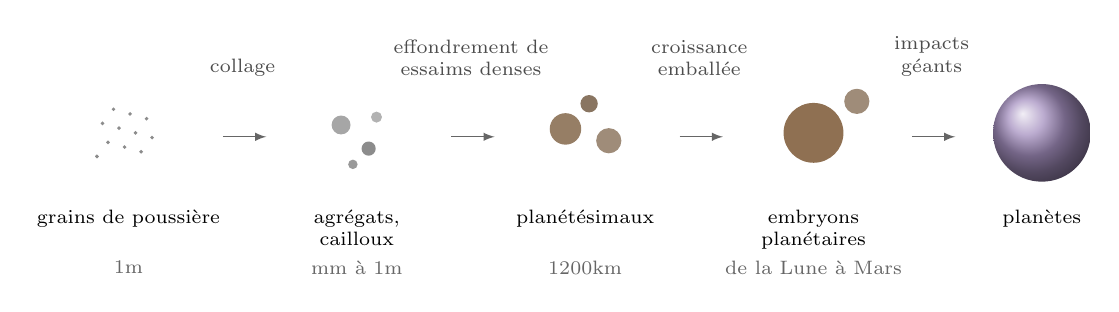
\begin{tikzpicture}[x=1cm, y=1cm, font=\scriptsize]
\foreach \x/\t/\s in {0/{grains de poussière}/{\qty{1}{\micro m}},
  2.9/{agrégats,\\cailloux}/{mm à \qty{1}{m}},
  5.8/{planétésimaux}/{\qtyrange{1}{200}{km}},
  8.7/{embryons\\planétaires}/{de la Lune à Mars},
  11.6/{planètes}/{} } {
  \node[align=center, anchor=north] at (\x,-0.9) {\t};
  \node[align=center, anchor=north, black!60] at (\x,-1.55) {\s};
}
\foreach \i in {0,...,11} {\fill[black!45] ({-0.4+0.07*mod(\i*7,11)},{-0.35+0.06*mod(\i*5,11)}) circle (0.025);}
\fill[black!35] (2.7,0.05) circle (0.12); \fill[black!45] (3.05,-0.25) circle (0.09);
\fill[black!40] (2.85,-0.45) circle (0.06); \fill[black!30] (3.15,0.15) circle (0.07);
\fill[brown!55!black!70] (5.55,0) circle (0.2); \fill[brown!50!black!60] (6.1,-0.15) circle (0.16);
\fill[brown!45!black!70] (5.85,0.32) circle (0.11);
\fill[brown!60!black!80] (8.7,-0.05) circle (0.38); \fill[brown!50!black!60] (9.25,0.35) circle (0.16);
\shade[ball color=blue!45!brown!60] (11.6,-0.05) circle (0.62);
\foreach \x in {1.2,4.1,7.0,9.95} {\draw[-latex, black!60] (\x,-0.1) -- +(0.55,0);}
  \node[align=center, anchor=south, black!70] at (1.45,0.55) {collage};
  \node[align=center, anchor=south, black!70] at (4.35,0.55) {effondrement de\\essaims denses};
  \node[align=center, anchor=south, black!70] at (7.25,0.55) {croissance\\emballée};
  \node[align=center, anchor=south, black!70] at (10.2,0.55) {impacts\\géants};
\end{tikzpicture}

\par\smallskip{\small Du grain de poussière aux planètes dans la région des planètes rocheuses (schéma, non à
l'échelle). Les grains s'agglomèrent en agrégats~; les essaims de cailloux s'effondrent en \omterm{def:b2:planet-formation-meteorites:planetesimal}{planétésimaux}~;
l'emballement gravitationnel fait passer certains \omterm{def:b2:planet-formation-meteorites:planetesimal}{planétésimaux} au rang d'embryons, qui finissent par fusionner
en planètes. Au-delà de la \omterm{def:b2:planet-formation-meteorites:snow-line}{ligne des glaces}, les embryons ont grandi davantage et ont pu capter du gaz. Tailles
d'après Chiang et Youdin (2010) et Lugaro et al. (2018).}
% ledger: cy10:growth, lugaro:cai
\end{omfigure}

Les planètes n'ont guère conservé la mémoire de cette histoire~: elles ont fondu, se sont mélangées et ont
remanié leur matière. Les archives se trouvent dans les corps qui ont cessé de croître, les astéroïdes, et dans
les morceaux de ceux-ci qui atteignent la Terre.

\section{Météorites}

\begin{definition}[Météorite, chute de météorite, trouvaille de météorite]
\label{def:b2:planet-formation-meteorites:fall-find}
Une \emph{météorite}\index{météorite} est un objet solide naturel venu de l'espace, qui
a survécu à sa traversée de l'atmosphère et atteint le sol. Une \emph{chute de
météorite}\index{chute de météorite} est une météorite recueillie après que son arrivée
a été observée, en général sous forme de bolide~; une \emph{trouvaille de
météorite}\index{trouvaille de météorite} est une météorite reconnue au sol sans que sa
chute ait été vue.
\end{definition}

La Terre balaie bien plus de poussière que de pierres. Mesurée dans la neige du plateau
antarctique, environ \qty{5200}{t} de poussière extraterrestre atteignent le sol chaque année
sous forme de micrométéorites et de sphérules fondues, sur quelque \qty{15000}{t} qui entrent
dans l'atmosphère, cette poussière provenant surtout des comètes et pour environ un cinquième
des astéroïdes. Les \omterm{def:b2:planet-formation-meteorites:fall-find}{météorites}, c'est-à-dire les pierres et les fers assez gros pour être
reconnus un à un, sont moins nombreuses~: le catalogue mondial en recense environ \num{45000},
dont seules \num{1107} sont des chutes.
% ledger: rojas21:flux, data:b4-meteorites

La distinction compte. Une chute est recueillie en quelques jours, avant que la pluie et l'oxygène ne
l'aient altérée, et toutes les sortes de \omterm{def:b2:planet-formation-meteorites:fall-find}{météorites} qui tombent sont recueillies de la même façon~; une
trouvaille peut être restée au sol pendant des milliers d'années, et sa chance d'être trouvée dépend de
son aspect et de l'endroit où elle est tombée. La moitié de toutes les trouvailles ont été faites en
Antarctique (encadré ci-dessous), où la recherche est systématique. Les chutes constituent l'échantillon
le plus équitable de ce qui arrive (figure ci-dessous)~: plus de quatre sur cinq sont des \omterm{def:b2:planet-formation-meteorites:chondrule}{chondrites}, et
trois sur quatre des \omterm{def:b2:planet-formation-meteorites:chondrule}{chondrites} ordinaires.
% ledger: data:b4-meteorites

\begin{omfigure}
\begin{tikzpicture}
\begin{axis}[width=0.86\linewidth, height=6.3cm, ybar, bar width=7pt,
  xmin=0.4, xmax=9.6, ymin=0.1, ymax=200, ymode=log, log origin=infty,
  xtick={1,...,9}, xticklabels={ordinaires, carbonées, enstatites, autres chondrites,
    HED, autres achondrites, fer, mixte, non classées},
  x tick label style={font=\scriptsize, rotate=30, anchor=north east, inner sep=1pt},
  tick label style={font=\scriptsize}, label style={font=\small},
  ylabel={part de l'échantillon (\%)}, legend pos=north east, xtick pos=bottom,
  legend style={font=\scriptsize, draw=black!30}, ymajorgrids, grid style={black!12}]
\addplot[fill=orange!70, draw=none] table[x=idx, y=falls_pct] {figdata/out/bachelor-2-meteorites-frac.dat};
\addlegendentry{chutes (\num{1107})}
\addplot[fill=blue!45, draw=none] table[x=idx, y=finds_pct] {figdata/out/bachelor-2-meteorites-frac.dat};
\addlegendentry{trouvailles (\num{44534})}
\end{axis}
\end{tikzpicture}

\par\smallskip{\small \omterm{def:b2:planet-formation-meteorites:fall-find}{Météorites} par classe, en pourcentage des chutes et des
trouvailles (échelle logarithmique)~; HED~: howardites, eucrites et diogénites.
Données~: export NASA de la Meteoritical Bulletin Database de The Meteoritical
Society (\num{45641} \omterm{def:b2:planet-formation-meteorites:fall-find}{météorites} valides).}
% ledger: data:b4-meteorites
\end{omfigure}

\begin{inthefield}[Recherche de météorites sur la glace bleue]
\begin{minipage}[t]{0.6\linewidth}\vspace{0pt}
La plus grande partie de la calotte glaciaire antarctique est une neige blanche, mais sur
environ \qty{1}{\percent} de sa surface, là où des montagnes bloquent l'écoulement de la glace,
environ \qty{5}{cm} de glace disparaissent chaque année et de la glace bleue nue apparaît. Les
\omterm{def:b2:planet-formation-meteorites:fall-find}{météorites} tombées sur la neige en amont, au cours de dizaines de milliers d'années, sont
enfouies, entraînées dans la glace et ramenées à la surface là où elle fond~: la glace bleue est
un piège. Depuis le début de la collecte systématique, au milieu des années 1970, les équipes
ont récupéré plus de \num{30000} spécimens dans de tels champs, et dans le catalogue la moitié
de toutes les trouvailles proviennent du sud de \ang{60}\,S. Les chercheurs traversent la glace
en lignes, à pied ou en motoneige, et chaque pierre trouvée est recueillie, quelle que soit son
apparence banale, de sorte que la collection ne penche pas vers les pièces spectaculaires.
Chaque trouvaille est photographiée à l'endroit où elle gît, pour enregistrer son contexte, et
reçoit un numéro de terrain~; plus tard elle reçoit son nom officiel, un code de trois lettres
pour le champ de glace suivi de l'année de la campagne et d'un numéro de série. Au laboratoire
de conservation, les pierres sont prélevées par éclats à l'aide d'outils en acier inoxydable, ou
découpées à sec à la scie à ruban~; les \omterm{def:b2:planet-formation-meteorites:chondrule}{chondrites carbonées}, qui peuvent renfermer des composés
organiques, ont leur propre armoire depuis 1978.
\end{minipage}\hfill
\begin{minipage}[t]{0.37\linewidth}\vspace{0pt}
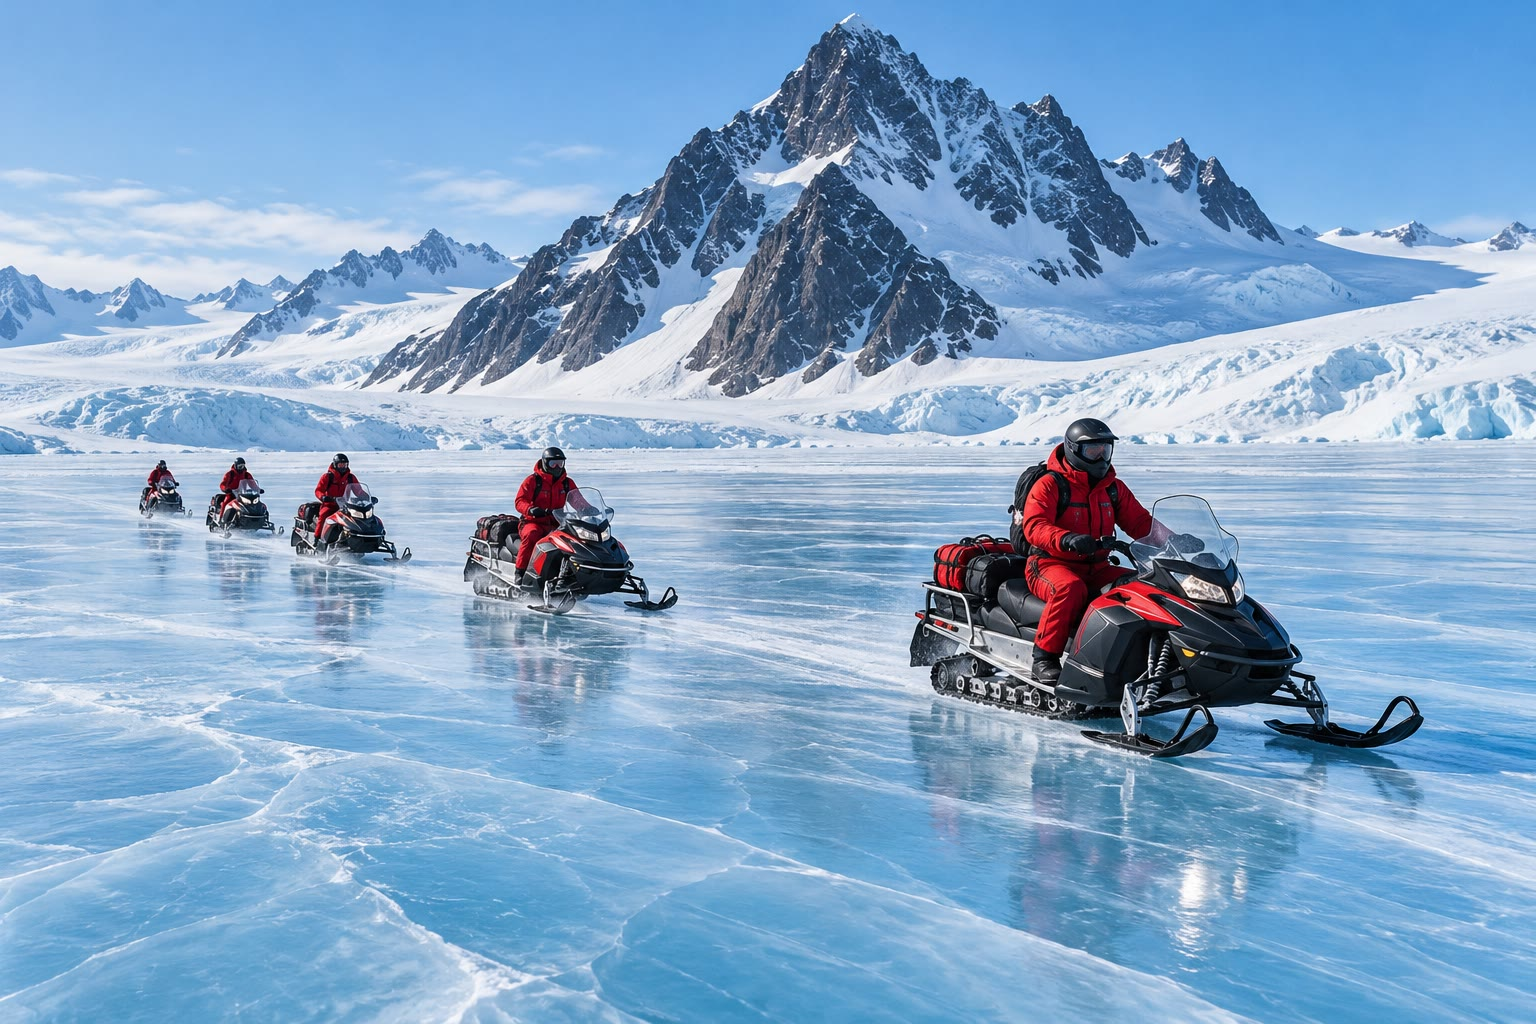
\includegraphics[width=\linewidth]{images/book4/ai/b2-blue-ice-search.jpg}

{\scriptsize Une file de chercheurs en motoneige traversant un champ de glace bleue au pied d'un pic
rocheux (Illustration générée par IA).}
\end{minipage}
% ledger: folco06:blue-ice, data:b4-meteorites, nasa:antmet
\end{inthefield}

\subsection{Chondrites}

\begin{definition}[Chondrite, chondrite carbonée, chondre, CAI]
\label{def:b2:planet-formation-meteorites:chondrule}
Une \emph{chondrite}\index{chondrite} est une \omterm{def:b2:planet-formation-meteorites:fall-find}{météorite} pierreuse qui n'a jamais fondu après
son assemblage, et dont la composition, à l'exception des éléments les plus volatils, est
proche de celle du Soleil. Elle est en grande partie faite de
\emph{chondres}\index{chondre}, de petites gouttelettes arrondies, d'un dixième de
millimètre à environ un centimètre de diamètre, de roche silicatée solidifiée à partir d'un
liquide, prises dans une matrice à grain fin avec des grains de métal fer--nickel et de
sulfure de fer. Certaines chondrites renferment des \emph{inclusions riches en calcium et
aluminium}\index{inclusion riche en calcium et aluminium} (CAI), grains blancs irréguliers
de minéraux de calcium, d'aluminium et de titane, qui sont les premiers condensats de la
nébuleuse. Une \emph{chondrite carbonée}\index{chondrite carbonée} est une chondrite riche
en carbone, en minéraux hydratés et en matrice, dont la teneur en éléments volatils est la
plus proche de celle du Soleil.
\end{definition}

Les \omterm{def:b2:planet-formation-meteorites:chondrule}{chondres} ont été fondus pendant quelques minutes seulement et refroidis en quelques heures à
quelques jours~: un bref chauffage local et instantané dans la nébuleuse, dont la cause reste inconnue,
a fondu des amas de poussière, qui se sont figés en gouttelettes avant d'être réunis, avec la poussière
et le métal, en un \omterm{def:b2:planet-formation-meteorites:planetesimal}{planétésimal}. Ils constituent jusqu'à \qty{90}{\percent} du volume des \omterm{def:b2:planet-formation-meteorites:fall-find}{météorites}
les plus primitives. Les CAI représentent de moins de \qty{1}{\percent} des \omterm{def:b2:planet-formation-meteorites:chondrule}{chondrites} ordinaires à
plus de \qty{10}{\percent} de certaines \omterm{def:b2:planet-formation-meteorites:chondrule}{chondrites carbonées}, et ils se sont formés à une centaine de
milliers d'années près les uns des autres.
% ledger: gail:meteorites, cy10:growth, cy10:chondrules, gail:chondrite-table, lugaro:cai

\begin{omfigure}
\begin{minipage}[c]{0.5\linewidth}
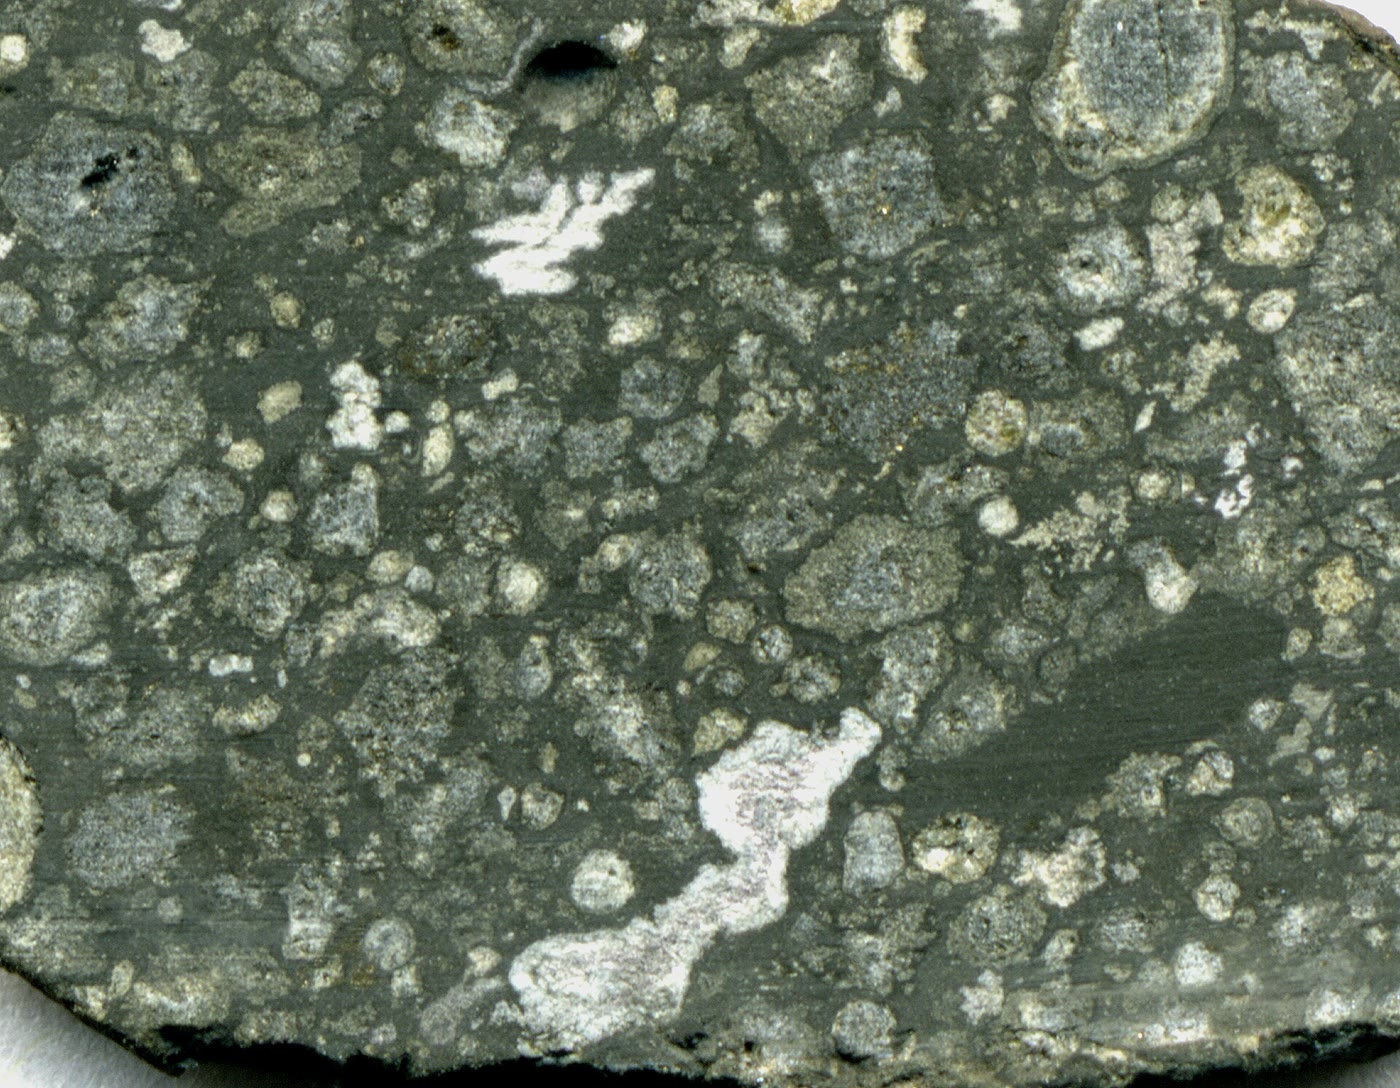
\includegraphics[width=\linewidth]{images/book4/b2-allende-chondrite.jpg}
\end{minipage}\hfill
\begin{minipage}[c]{0.46\linewidth}
{\small Face sciée de la \omterm{def:b2:planet-formation-meteorites:chondrule}{chondrite carbonée} d'Allende (classe CV3), tombée dans le nord du Mexique en
1969~: environ deux tonnes ont été recueillies. Les grains gris arrondis sont des \omterm{def:b2:planet-formation-meteorites:chondrule}{chondres}~; les
taches blanches irrégulières sont des CAI~; le ciment sombre est la matrice. La vue couvre quelques
centimètres de large. James St.\ John, CC BY 2.0.}
\end{minipage}
% ledger: data:b4-meteorites, gail:chondrite-table
\end{omfigure}

Les \omterm{def:b2:planet-formation-meteorites:chondrule}{chondrites} se répartissent en groupes qui diffèrent par la taille et l'abondance de
leurs \omterm{def:b2:planet-formation-meteorites:chondrule}{chondres}, leur teneur en métal, la teneur en fer de leur olivine et la proportion
de leur matrice (tableau ci-dessous). Les \omterm{def:b2:planet-formation-meteorites:chondrule}{chondrites} ordinaires H, L et LL ont des
teneurs en métal et en fer total élevée, faible et très faible (rapports atomiques Fe/Si
de \num{0.80}, \num{0.59} et \num{0.53}).
% ledger: gail:chondrite-table

\begin{table}[h]
\centering
\small
\begin{tabular}{lcccccc}
\hline
 & H & L & LL & CI & CM & CV\\
\hline
\omterm{def:b2:planet-formation-meteorites:chondrule}{chondres} (vol.\ \%) & 60--80 & 60--80 & 60--80 & $\ll 1$ & 20 & 45\\
diamètre moyen des \omterm{def:b2:planet-formation-meteorites:chondrule}{chondres} (mm) & 0.3 & 0.7 & 0.9 & --- & 0.3 & 1.0\\
CAI (vol.\ \%) & 0.1--1 & 0.1--1 & 0.1--1 & $\ll 1$ & 5 & 10\\
matrice (vol.\ \%) & 10--15 & 10--15 & 10--15 & $> 99$ & 70 & 40\\
métal fer--nickel (vol.\ \%) & 10 & 5 & 2 & 0 & 0.1 & 0--5\\
fayalite dans l'olivine (mol \%) & 16--20 & 23--26 & 27--32 & & & \\
\omterm{def:b2:planet-formation-meteorites:type}{types pétrologiques} & 3--6 & 3--6 & 3--6 & 1 & 2 & 3\\
température maximale (K) & 1220 & 1220 & 1220 & 430 & 670 & 870\\
\hline
\end{tabular}
\caption{Propriétés des \omterm{def:b2:planet-formation-meteorites:chondrule}{chondrites} ordinaires (H, L, LL) et de trois groupes de \omterm{def:b2:planet-formation-meteorites:chondrule}{chondrites carbonées}. Fayalite~: le pôle riche en fer
de l'olivine. Données~: Gail et al. (2014).}
\label{tab:b2:planet-formation-meteorites:chondrites}
% ledger: gail:chondrite-table
\end{table}

\begin{definition}[Type pétrologique]\label{def:b2:planet-formation-meteorites:type}
Le \emph{type pétrologique}\index{type pétrologique} d'une \omterm{def:b2:planet-formation-meteorites:chondrule}{chondrite} est un nombre de 1 à 6 qui
enregistre ce qui lui est arrivé dans son corps parent~: le type 3 est le moins altéré~; les
types 4 à 6 sont de plus en plus chauffés, leurs \omterm{def:b2:planet-formation-meteorites:chondrule}{chondres} estompés et leurs minéraux
recristallisés, de composition uniforme~; les types 2 et 1 sont de plus en plus altérés par
l'eau liquide, qui a transformé leurs minéraux en argiles.
\end{definition}

La dernière ligne du tableau donne les températures les plus élevées atteintes par chaque groupe~: jusqu'à
environ \qty{1220}{K} pour les \omterm{def:b2:planet-formation-meteorites:chondrule}{chondrites} ordinaires les plus chauffées, jamais plus de \qty{430}{K} pour les
\omterm{def:b2:planet-formation-meteorites:chondrule}{chondrites} CI, imprégnées d'eau mais jamais chaudes. La chaleur, comme le montre la dernière section,
provenait de l'intérieur des corps parents.
% ledger: gail:chondrite-table

\subsection{Achondrites et fers}

\begin{definition}[Achondrite, météorite de fer, météorite mixte]
\label{def:b2:planet-formation-meteorites:classes}
Une \emph{achondrite}\index{achondrite} est une \omterm{def:b2:planet-formation-meteorites:fall-find}{météorite} pierreuse qui a
cristallisé à partir d'un liquide, ou recristallisé à haute température dans un
corps qui a fondu, et qui ne contient donc pas de \omterm{def:b2:planet-formation-meteorites:chondrule}{chondres}. Une \emph{météorite de
fer}\index{météorite de fer} est faite surtout d'alliage métallique fer--nickel. Une
\emph{météorite mixte}\index{météorite mixte} est faite de métal et de silicate en
quantités à peu près égales.
\end{definition}

Ce sont les morceaux de corps qui ont fondu et se sont séparés~: les \omterm{def:b2:planet-formation-meteorites:classes}{achondrites} sont
leurs croûtes et leurs manteaux, les fers leurs noyaux métalliques, et les mixtes
proviennent de la zone où métal et silicate se sont rencontrés. La plus grande famille
d'\omterm{def:b2:planet-formation-meteorites:classes}{achondrites}, celle des howardites, eucrites et diogénites (HED), basaltes et roches
riches en pyroxène, représente \qty{5.5}{\percent} de toutes les chutes. Son origine a
été rattachée, par son spectre et son orbite, à l'astéroïde Vesta, d'environ
\qty{525}{km} de diamètre, et la sonde Dawn, qui a atteint Vesta en 2011, l'a confirmé~:
la chimie et la minéralogie de la surface de Vesta correspondent aux \omterm{def:b2:planet-formation-meteorites:fall-find}{météorites} HED, un
bassin de \qty{500}{km} de large près de son pôle Sud montre d'où les fragments ont été
arrachés, et son champ de gravité indique un noyau de fer d'environ \qty{225}{km} de
diamètre. Vesta a fondu, en partie ou en totalité, tôt dans son histoire. D'autres
\omterm{def:b2:planet-formation-meteorites:classes}{achondrites} viennent de la Lune et de Mars. Les \omterm{def:b2:planet-formation-meteorites:fall-find}{météorites} des collections semblent
provenir d'une centaine de corps parents différents.
% ledger: data:b4-meteorites, nasa:vesta-dawn, gail:meteorites

Les \omterm{def:b2:planet-formation-meteorites:classes}{météorites de fer} gardent la trace du refroidissement de leurs noyaux. Une face sciée puis attaquée
à l'acide montre un entrecroisement de plaquettes (figure ci-dessous)~: à haute température, le métal
est un alliage unique de fer et de nickel~; au refroidissement lent, un alliage pauvre en nickel croît
en plaquettes le long des plans du cristal d'origine, et plus le refroidissement est lent, plus les
plaquettes sont larges. Mesurée sur de nombreux fers, la largeur des plaquettes donne les vitesses de
refroidissement des noyaux dont ils proviennent.
% ledger: gail:meteorites

\begin{omfigure}
\begin{minipage}[c]{0.5\linewidth}
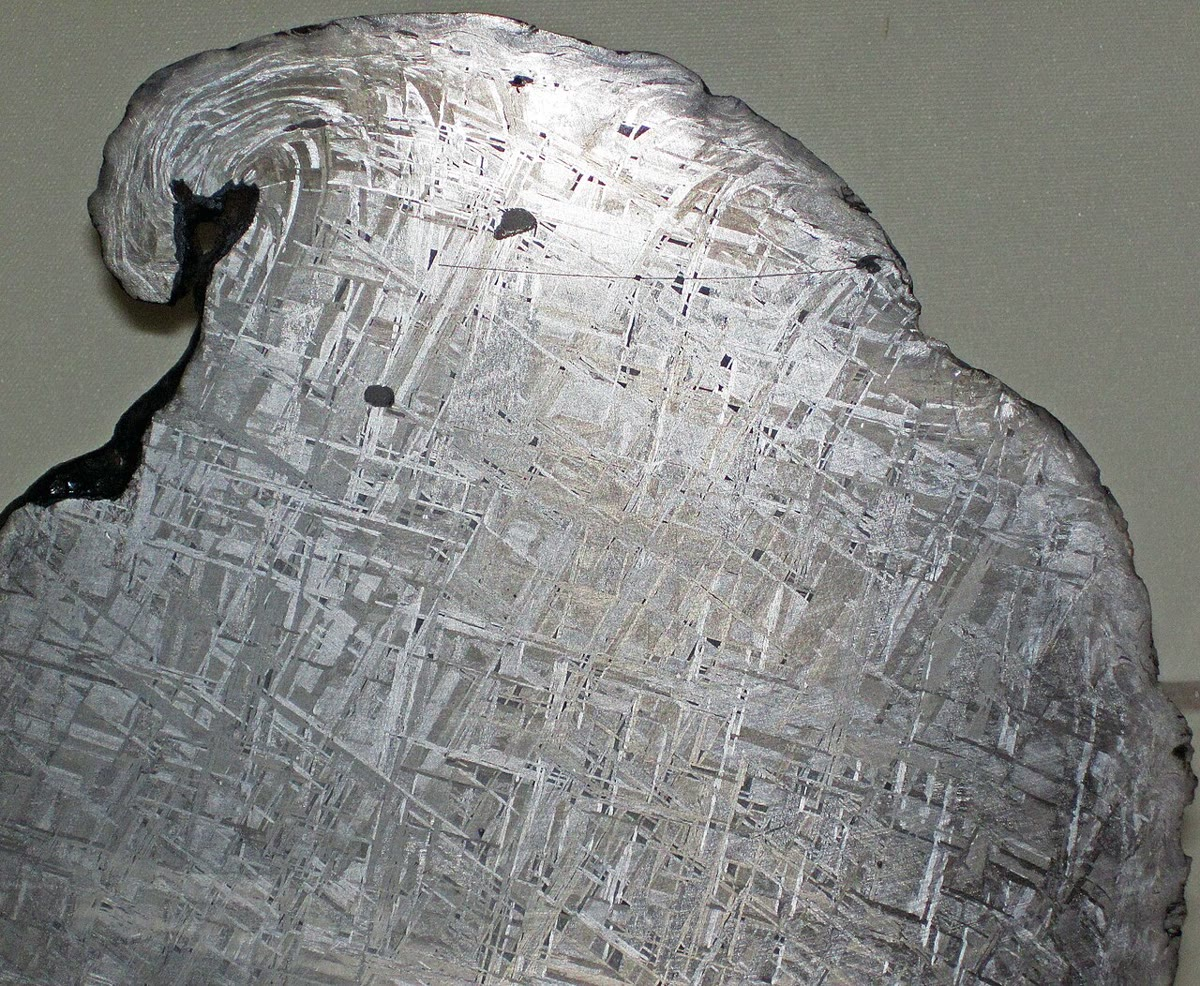
\includegraphics[width=\linewidth]{images/book4/b2-gibeon-widmanstatten.jpg}
\end{minipage}\hfill
\begin{minipage}[c]{0.46\linewidth}
{\small La face sciée, polie et attaquée à l'acide d'un fragment de la \omterm{def:b2:planet-formation-meteorites:classes}{météorite de fer} de
Gibeon, trouvée en Namibie~: l'entrecroisement de plaquettes d'alliage fer--nickel (figure de
Widmanstätten) s'est formé pendant le refroidissement lent du noyau métallique de son corps
parent. James St.\ John, CC BY 2.0.}
\end{minipage}
% ledger: data:b4-meteorites
\end{omfigure}

\section{Dater le système solaire}

L'âge du système solaire est celui de ses plus vieux solides. Les isochrones
uranium--plomb des CAI, construits comme dans le volume de première année, donnent
\qtyrange{4567}{4568}{\Ma}~; les CAI se sont formés à \qty{0.1}{Ma} près les uns des
autres, un intervalle assez court pour que leur âge soit pris pour la naissance du Soleil.
Les événements des quelques millions d'années suivantes, la formation des \omterm{def:b2:planet-formation-meteorites:chondrule}{chondres} et
l'assemblage puis la fusion des premiers corps, se datent au mieux par rapport aux CAI, à
l'aide d'horloges qui ont tourné vite et se sont arrêtées tôt.
% ledger: lugaro:cai

\begin{definition}[Radionucléide de courte période]
\label{def:b2:planet-formation-meteorites:slr}
Un \emph{radionucléide de courte période}\index{radionucléide de courte période} est
un nucléide radioactif dont la demi-vie est d'environ \num{0.1} à \qty{100}{Ma},
présent lorsque le système solaire s'est formé et aujourd'hui éteint, et dont la
présence passée se révèle par un excès de son nucléide fils dans des minéraux riches
en son élément.
\end{definition}

Le plus connu est l'aluminium 26, qui se désintègre en magnésium 26 avec une demi-vie
de \qty{0.717}{Ma} (une durée de vie moyenne de \qty{1.035}{Ma}). Lorsque les CAI se
sont formés, un atome d'aluminium sur environ \num{19000} était de l'aluminium 26~: le
rapport $\ce{^{26}Al}/\ce{^{27}Al}$ valait $(5.23 \pm 0.13)\times10^{-5}$, la valeur
\emph{canonique}. Les autres nucléides de courte période couvrent des durées plus
longues (tableau ci-dessous).
% ledger: lugaro:al26, lugaro:slr-table

\begin{table}[h]
\centering
\small
\begin{tabular}{lllcc}
\hline
nucléide & fils & référence & demi-vie (Ma) & rapport initial\\
\hline
\ce{^{26}Al} & \ce{^{26}Mg} & \ce{^{27}Al} & 0.717 & $5.23\times10^{-5}$\\
\ce{^{60}Fe} & \ce{^{60}Ni} & \ce{^{56}Fe} & 2.62 & $1.0\times10^{-8}$\\
\ce{^{53}Mn} & \ce{^{53}Cr} & \ce{^{55}Mn} & 3.74 & $7\times10^{-6}$\\
\ce{^{107}Pd} & \ce{^{107}Ag} & \ce{^{108}Pd} & 6.5 & $6.6\times10^{-5}$\\
\ce{^{182}Hf} & \ce{^{182}W} & \ce{^{180}Hf} & 8.90 & $1.02\times10^{-4}$\\
\ce{^{129}I} & \ce{^{129}Xe} & \ce{^{127}I} & 15.7 & $1.28\times10^{-4}$\\
\hline
\end{tabular}
\caption{Quelques \omterm{def:b2:planet-formation-meteorites:slr}{radionucléides de courte période} du système solaire primitif,
leur nucléide fils stable, l'isotope stable du même élément pris comme référence,
leur demi-vie et leur rapport à la référence lorsque les CAI se sont formés.
Données~: Lugaro et al. (2018).}
\label{tab:b2:planet-formation-meteorites:slr}
% ledger: lugaro:al26, lugaro:slr-table
\end{table}

\begin{proposition}[Âge relatif à partir d'un nucléide éteint]
\label{prop:b2:planet-formation-meteorites:relative-age}
Si le rapport d'un nucléide de courte période à son isotope de référence valait $R_0$
partout lorsque les CAI se sont formés, et s'il est trouvé égal à $R$ dans un objet au
moment de sa formation, l'objet s'est formé
\[
  \Delta t = \tau \ln\frac{R_0}{R}
\]
après les CAI, où $\tau$ est la durée de vie moyenne du nucléide. Une erreur $\delta R$ sur $R$ donne l'erreur
$\tau\,\delta R/R$ sur $\Delta t$.
\end{proposition}

\begin{proof}
L'isotope de référence est stable, si bien que le rapport décroît comme le nucléide radioactif
lui-même~: $R = R_0 e^{-\Delta t/\tau}$. En prenant les logarithmes,
$\Delta t = \tau\ln(R_0/R)$. En dérivant, $\mathrm d(\Delta t) =
-\tau\,\mathrm dR/R$.
\end{proof}

Une erreur relative de \qty{10}{\percent} sur le rapport coûte ainsi \qty{0.1}{Ma}
avec l'aluminium 26, mais \qty{0.54}{Ma} avec le manganèse 53 et \qty{1.3}{Ma} avec
l'hafnium 182~: chaque horloge n'est précise que sur quelques-unes de ses propres
durées de vie moyennes, et la bonne horloge dépend de l'événement. Le rapport $R$ dans
un objet se lit sur ses minéraux.
% ledger: lugaro:al26, lugaro:slr-table

\begin{proposition}[Isochrone aluminium--magnésium]
\label{prop:b2:planet-formation-meteorites:al-mg}
Soient plusieurs minéraux d'un même objet qui se forment ensemble à l'instant $\Delta t$ avec la
même composition isotopique du magnésium, $(\ce{^{26}Mg}/\ce{^{24}Mg})_0$, mais des rapports
$\ce{^{27}Al}/\ce{^{24}Mg}$ différents, et qui restent fermés depuis. Aujourd'hui ils se placent
sur la droite
\[
  \frac{\ce{^{26}Mg}}{\ce{^{24}Mg}}
  = \left(\frac{\ce{^{26}Mg}}{\ce{^{24}Mg}}\right)_0
  + R\,\frac{\ce{^{27}Al}}{\ce{^{24}Mg}},
\]
dont la pente est le rapport $R = \ce{^{26}Al}/\ce{^{27}Al}$ de l'objet au
moment de sa formation.
\end{proposition}

\begin{proof}
Chaque atome d'aluminium 26 présent à la formation est devenu depuis un atome
de magnésium 26, si bien qu'un minéral a gagné
$\ce{^{26}Al}_{\text{alors}} = R\,\ce{^{27}Al}$ atomes de magnésium 26,
l'aluminium 27 étant stable. En divisant par le nombre d'atomes de magnésium
24, qui ne change pas, on obtient la droite.
\end{proof}

Les minéraux riches en aluminium et pauvres en magnésium, comme le plagioclase, montrent de
forts excès de magnésium 26~; l'olivine, presque dépourvue d'aluminium, n'en montre aucun.
C'est ainsi qu'a été construite la chronologie du système solaire primitif~: d'abord les
CAI, puis les \omterm{def:b2:planet-formation-meteorites:chondrule}{chondres} pendant les quelques millions d'années suivantes, les indices
fournis par les \omterm{def:b2:planet-formation-meteorites:chondrule}{chondres} fixant la durée de vie du disque de gaz à moins de cinq millions
d'années~; les corps parents des \omterm{def:b2:planet-formation-meteorites:chondrule}{chondrites} se sont assemblés après leurs \omterm{def:b2:planet-formation-meteorites:chondrule}{chondres} les plus
jeunes. Les diogénites, roches du manteau de Vesta, ont commencé à cristalliser dans le
million d'années environ qui a suivi les CAI, et le noyau de Vesta s'est formé entre le
premier et le quatrième million d'années~: les \omterm{def:b2:planet-formation-meteorites:classes}{météorites de fer} et les \omterm{def:b2:planet-formation-meteorites:classes}{achondrites} sont
plus vieilles que beaucoup de \omterm{def:b2:planet-formation-meteorites:chondrule}{chondrites}.
% ledger: lugaro:cai, gail:vesta, gail:meteorites

\section{La chaleur de l'aluminium 26 et les premières fusions}

D'où venait la chaleur qui a fondu Vesta et métamorphisé les \omterm{def:b2:planet-formation-meteorites:chondrule}{chondrites} ordinaires~? Modèles et \omterm{def:b2:planet-formation-meteorites:fall-find}{météorites}
s'accordent sur le fait que, dans les corps les plus anciens, la source dominante était la désintégration de
l'aluminium 26. Dans une roche de composition chondritique, elle portait au départ \qty{5}{MJ} par kilogramme,
disponibles pour être libérés en quelques millions d'années~: assez pour chauffer la roche de plusieurs milliers
de kelvins, si la chaleur ne pouvait pas s'échapper.
% ledger: lugaro:heat, lugaro:melting

\begin{proposition}[Chauffage d'un planétésimal par l'aluminium 26]
\label{prop:b2:planet-formation-meteorites:heating}
Une roche qui reçoit la puissance radioactive $H_0 e^{-t/\tau}$ par kilogramme, de
capacité thermique massique $c$, et qui ne perd pas de chaleur, s'échauffe après son
accrétion, à l'instant $t_a$, selon
\[
  T(t) = T_0 + \frac{H_0\tau}{c}\left(e^{-t_a/\tau} - e^{-t/\tau}\right),
\]
et tend vers la température maximale
$T_{\max} = T_0 + (H_0\tau/c)\,e^{-t_a/\tau}$. Une température critique
$T_c > T_0$ n'est atteinte que si le corps s'est accrété avant
\[
  t_a^* = \tau\ln\frac{H_0\tau}{c\,(T_c - T_0)}.
\]
\end{proposition}

\begin{proof}
Sans pertes, $c\,\mathrm dT/\mathrm dt = H_0 e^{-t/\tau}$. En intégrant à partir de $t_a$,
où $T = T_0$, on obtient $c\,(T - T_0) = H_0\tau\,(e^{-t_a/\tau} - e^{-t/\tau})$, qui tend
vers $H_0\tau e^{-t_a/\tau}$ lorsque $t \to \infty$. En posant $T_{\max} = T_c$ et en
résolvant pour $t_a$ on obtient $t_a^*$~; pour une accrétion plus précoce, le maximum est
plus élevé.
\end{proof}

Un modèle du corps parent des \omterm{def:b2:planet-formation-meteorites:chondrule}{chondrites} ordinaires utilise
$H_0 = \qty{1.9e-7}{W.kg^{-1}}$, $c = \qty{837}{J.kg^{-1}.K^{-1}}$ et
$T_0 = \qty{250}{K}$. Alors $H_0\tau/c$ vaut environ \qty{7400}{K}. Trois températures
comptent~: vers \qty{750}{K}, la roche poreuse commence à se compacter par frittage~;
vers \qty{1200}{K}, le métal et le sulfure de fer commencent à fondre ensemble~; vers
\qty{1700}{K}, les derniers silicates fondent. Un corps accrété avant \qty{1.7}{Ma} a
entièrement fondu~; avant \qty{2.1}{Ma}, son métal et son sulfure ont fondu et ont pu
descendre former un noyau~; jusqu'à environ \qty{2.8}{Ma}, il a au moins été fritté et
métamorphisé~; les corps plus tardifs sont restés froids (figure ci-dessous).
% ledger: gail:params, gail:temps, lugaro:al26

\begin{omfigure}
\begin{tikzpicture}
\begin{axis}[omrecord, name=left, width=0.45\linewidth, height=6.0cm,
  xmin=0, xmax=8, ymin=0, ymax=2300,
  xlabel={temps après les CAI (Ma)}, ylabel={température (K)},
  tick label style={font=\scriptsize}, label style={font=\small}]
\addplot[black!45, densely dashed, domain=0:8, samples=2] {750};
\addplot[black!45, densely dashed, domain=0:8, samples=2] {1200};
\addplot[black!45, densely dashed, domain=0:8, samples=2] {1700};
\addplot[thick, red!75!black] table[x=t_Myr, y=T_K] {figdata/out/bachelor-2-al26-ta15.dat};
\addplot[thick, orange!80!black] table[x=t_Myr, y=T_K] {figdata/out/bachelor-2-al26-ta20.dat};
\addplot[thick, teal!70!black] table[x=t_Myr, y=T_K] {figdata/out/bachelor-2-al26-ta25.dat};
\addplot[thick, blue!70!black] table[x=t_Myr, y=T_K] {figdata/out/bachelor-2-al26-ta30.dat};
\node[font=\tiny, red!75!black, anchor=south east] at (axis cs:7.9,1995) {$t_a = \qty{1.5}{Ma}$};
\node[font=\tiny, orange!80!black, anchor=south east] at (axis cs:7.9,1325) {2};
\node[font=\tiny, teal!70!black, anchor=south east] at (axis cs:7.9,915) {2.5};
\node[font=\tiny, blue!70!black, anchor=north east] at (axis cs:7.9,650) {3};
\node[font=\tiny, black!60, anchor=south west] at (axis cs:0.1,1700) {silicates fondus};
\node[font=\tiny, black!60, anchor=south west] at (axis cs:0.1,1200) {Fe--FeS fond};
\node[font=\tiny, black!60, anchor=south west] at (axis cs:0.1,750) {frittage};
\end{axis}
\begin{axis}[omrecord, at={(left.east)}, anchor=west, xshift=2.1cm, width=0.45\linewidth,
  height=6.0cm, xmin=0, xmax=4, ymin=0, ymax=8000,
  xlabel={temps d'accrétion $t_a$ (Ma)}, ylabel={température maximale (K)},
  tick label style={font=\scriptsize}, label style={font=\small},
  scaled y ticks=false, yticklabel style={/pgf/number format/1000 sep={\,}}]
\addplot[black!45, densely dashed, domain=0:4, samples=2] {750};
\addplot[black!45, densely dashed, domain=0:4, samples=2] {1200};
\addplot[black!45, densely dashed, domain=0:4, samples=2] {1700};
\addplot[thick, black] table[x=ta_Myr, y=Tpeak_K] {figdata/out/bachelor-2-al26-peak.dat};
\draw[black!60] (axis cs:1.69,0) -- (axis cs:1.69,1700);
\draw[black!60] (axis cs:2.13,0) -- (axis cs:2.13,1200);
\node[font=\tiny, black!70, anchor=south] at (axis cs:2.0,4500) {\qty{1.7}{Ma}};
\draw[black!50, -latex] (axis cs:2.0,4450) -- (axis cs:1.71,1800);
\node[font=\tiny, black!70, anchor=south] at (axis cs:2.9,3300) {\qty{2.1}{Ma}};
\draw[black!50, -latex] (axis cs:2.9,3250) -- (axis cs:2.16,1300);
\end{axis}
\end{tikzpicture}

\par\smallskip{\small Chauffage de l'intérieur d'un corps chondritique par l'aluminium 26, sans perte de
chaleur (la proposition ci-dessus~; $H_0 = \qty{1.9e-7}{W.kg^{-1}}$, $c = \qty{837}{J.kg^{-1}.K^{-1}}$,
$T_0 = \qty{250}{K}$, $\tau = \qty{1.035}{Ma}$). À gauche~: température en fonction du temps pour des
corps accrétés \qty{1.5}{Ma}, 2, 2.5 et \qty{3}{Ma} après les CAI. À droite~: température maximale en
fonction du temps d'accrétion~; les corps accrétés avant \qty{1.7}{Ma} ont fondu, et ceux accrétés avant
\qty{2.1}{Ma} ont vu fondre leur métal et leur sulfure. Les corps réels consacrent une partie de la
chaleur à la fusion, ce qui plafonne la température, et perdent de la chaleur près de leur surface.
Valeurs du modèle~: Gail et al. (2014).}
% ledger: gail:params, gail:temps, lugaro:al26
\end{omfigure}

La proposition ignore les pertes de chaleur, qui ne valent que loin sous la surface d'un grand corps. La
chaleur diffuse sur la distance $\sqrt{\kappa t}$ pendant le temps $t$, où $\kappa$ est la diffusivité
thermique de la roche~: avec les valeurs du modèle, environ \qty{5}{km} pendant une durée de vie moyenne de
l'aluminium 26 (\cref{exo:b2:planet-formation-meteorites:12}). Les corps bien plus petits que cela perdent leur
chaleur aussi vite qu'ils la produisent~; des modèles détaillés montrent que les corps de plus de
\qtyrange{10}{20}{km} de diamètre pourraient fondre.
% ledger: gail:params, lugaro:melting

\begin{definition}[Différenciation planétaire]
\label{def:b2:planet-formation-meteorites:differentiation}
La \emph{différenciation planétaire}\index{différenciation planétaire} est la
séparation d'un corps, une fois fondu ou partiellement fondu, en couches de
composition et de densité différentes~: un noyau métallique, un manteau silicaté et
une croûte formée des derniers liquides de fusion.
\end{definition}

Les \omterm{def:b2:planet-formation-meteorites:fall-find}{météorites} conservent ainsi la trace de deux sortes de corps primitifs. Ceux qui se sont formés dans
les deux premiers millions d'années environ avaient assez d'aluminium 26 pour fondre et se
différencier~: leurs noyaux sont les \omterm{def:b2:planet-formation-meteorites:classes}{météorites de fer}, leurs croûtes et leurs manteaux les \omterm{def:b2:planet-formation-meteorites:classes}{achondrites},
et Vesta est le survivant. Ceux qui se sont formés plus tard sont restés des \omterm{def:b2:planet-formation-meteorites:chondrule}{chondrites}, chauffées de
l'intérieur à un degré fixé par leur date de naissance et par la profondeur de chaque fragment~: les
plus profonds sont devenus de type 6, et les moins profonds sont restés de type 3. La Terre elle-même,
construite à partir d'embryons et de \omterm{def:b2:planet-formation-meteorites:planetesimal}{planétésimaux} des deux sortes et frappée par des impacts géants,
s'est différenciée en noyau, manteau et croûte.
% ledger: gail:meteorites, gail:vesta, gail:temps

\section{Exercices}

\begin{exercise}[$\star$]\label{exo:b2:planet-formation-meteorites:1}
Dans la \omterm{def:b2:planet-formation-meteorites:nebula}{nébuleuse solaire} de masse minimale, calculer la densité surfacique du gaz à
\qty{1}{au} et à \qty{5.2}{au}, et celle des solides à \qty{1}{au} (roche seule,
$Z_{\mathrm{rel}} = 0.33$) et à \qty{5.2}{au} (toutes les glaces condensées,
$Z_{\mathrm{rel}} = 1$). Combien de fois le gaz est-il plus lourd que les solides à
\qty{5.2}{au}~?
% ledger: cy10:mmsn
\end{exercise}

\begin{exercise}[$\star$]\label{exo:b2:planet-formation-meteorites:2}
En utilisant la figure des \omterm{def:b2:planet-formation-meteorites:condensation}{températures de condensation}, classer l'aluminium, le sodium, le magnésium, le
fer, le soufre et l'oxygène (sous forme de glace d'eau), du premier au dernier à se condenser, et donner le
groupe de volatilité de chacun. Lesquels vous attendriez-vous à trouver enrichis dans les CAI, et lesquels
appauvris sur la Terre par rapport au Soleil~?
% ledger: lodders:tc-table, lodders:groups
\end{exercise}

\begin{exercise}[$\star$]\label{exo:b2:planet-formation-meteorites:3}
Le catalogue recense \num{1107} chutes, dont 856 \omterm{def:b2:planet-formation-meteorites:chondrule}{chondrites} ordinaires et 49 fers, et
\num{44534} trouvailles, dont \num{38647} \omterm{def:b2:planet-formation-meteorites:chondrule}{chondrites} ordinaires, \num{1020} fers et
\num{22096} venant du sud de \ang{60}\,S. Calculer la part des \omterm{def:b2:planet-formation-meteorites:chondrule}{chondrites} ordinaires et
celle des fers parmi les chutes et parmi les trouvailles, ainsi que la part des trouvailles
antarctiques. Quel échantillon utiliseriez-vous pour estimer les proportions dans lesquelles
les classes arrivent sur la Terre, et pourquoi~?
% ledger: data:b4-meteorites
\end{exercise}

\begin{exercise}[$\star$]\label{exo:b2:planet-formation-meteorites:4}
Les minéraux d'un objet donnent le rapport initial $\ce{^{26}Al}/\ce{^{27}Al} = \num{1.0e-5}$. Combien de
temps après les CAI cet objet s'est-il formé~? Prendre $R_0 = \num{5.23e-5}$ et une durée de vie moyenne
de \qty{1.035}{Ma}.
% ledger: lugaro:al26
\end{exercise}

\begin{exercise}[$\star\star$]\label{exo:b2:planet-formation-meteorites:5}
En utilisant la \cref{prop:b2:planet-formation-meteorites:disc-mass} avec
$\Sigma_1 = \qty{2.2e4}{kg.m^{-2}}$ à \qty{1}{au} (\qty{1}{au} $=
\qty{1.496e11}{m}$, $M_\odot = \qty{1.989e30}{kg}$), calculer la masse de la
nébuleuse de masse minimale à l'intérieur de \qty{30}{au} et de \qty{100}{au}, en
masses solaires. Comparer avec les disques observés, \numrange{0.001}{0.1} masse solaire.
% ledger: cy10:mmsn
\end{exercise}

\begin{exercise}[$\star\star$]\label{exo:b2:planet-formation-meteorites:6}
Dans le disque passif $T = \qty{120}{K}\,(r/\qty{1}{au})^{-3/7}$, déterminer où la glace d'eau
(\qty{182}{K}) et la glace de méthane (\qty{41}{K}) deviennent stables. Un grain en plein soleil atteint
\qty{182}{K} à \qty{2.3}{au}. Pourquoi les deux estimations de la \omterm{def:b2:planet-formation-meteorites:snow-line}{ligne des glaces} diffèrent-elles, et
laquelle s'applique aux corps qui ont construit les planètes~?
% ledger: cy10:passive, lodders:phases
\end{exercise}

\begin{exercise}[$\star\star$]\label{exo:b2:planet-formation-meteorites:7}
Calculer la masse d'isolement, avec $b = 5$, d'un embryon à \qty{1}{au} dans la nébuleuse de masse
minimale ($\Sigma_p = \qty{10.9}{g.cm^{-2}}$), et à \qty{5.2}{au} au-delà de la \omterm{def:b2:planet-formation-meteorites:snow-line}{ligne des glaces}
($\Sigma_p = \qty{2.78}{g.cm^{-2}}$), en masses terrestres ($M_\oplus = \qty{5.972e24}{kg}$,
$M_\odot = \qty{1.989e30}{kg}$). Que devient-elle à \qty{5.2}{au} dans un disque contenant \num{3.5}
fois plus de solides~?
% ledger: cy10:isolation, cy10:mmsn, earth:mass
\end{exercise}

\begin{exercise}[$\star\star$]\label{exo:b2:planet-formation-meteorites:8}
Une roche de composition CI contenait \num{1.01e16} atomes d'aluminium 26 par gramme
lorsque les CAI se sont formés, et chaque désintégration libère \qty{5.00e-13}{J} de
chaleur. Calculer la chaleur libérée par kilogramme au cours de toute la désintégration, et
l'élévation de température qu'elle donnerait avec $c = \qty{837}{J.kg^{-1}.K^{-1}}$ et sans
pertes. Combien de fois est-elle supérieure à la chaleur nécessaire pour chauffer la roche
de \num{250} à \qty{1700}{K}~?
% ledger: lugaro:heat, gail:params
\end{exercise}

\begin{exercise}[$\star\star$]\label{exo:b2:planet-formation-meteorites:9}
Sur toute sa désintégration, l'aluminium 26 libère \qty{5.07e10}{erg} par gramme de roche CI, et le fer 60
\qty{7.49e7}{erg} par gramme. Calculer le rapport des deux énergies. La demi-vie du fer 60 vaut
\qty{2.62}{Ma}~: calculer sa durée de vie moyenne, puis le rapport des deux puissances initiales de
chauffage, énergie divisée par durée de vie moyenne.
% ledger: lugaro:heat, lugaro:slr-table, lugaro:al26
\end{exercise}

\begin{exercise}[$\star\star\star$]\label{exo:b2:planet-formation-meteorites:10}
À partir des résultats de l'\cref{exo:b2:planet-formation-meteorites:9}, trouver le temps au-delà duquel le
fer 60 chauffe la roche plus vite que l'aluminium 26. Le fer 60 aurait-il pu fondre un corps accrété aussi
tard~? (Comparer l'énergie qui reste alors à libérer avec les \qty{1.2e6}{J.kg^{-1}} nécessaires pour
chauffer la roche de \num{250} à \qty{1700}{K}.)
% ledger: lugaro:heat, lugaro:slr-table, lugaro:al26
\end{exercise}

\begin{exercise}[$\star\star\star$]\label{exo:b2:planet-formation-meteorites:11}
Avec $H_0 = \qty{1.9e-7}{W.kg^{-1}}$, $\tau = \qty{1.035}{Ma}$,
$c = \qty{837}{J.kg^{-1}.K^{-1}}$ et $T_0 = \qty{250}{K}$ (une année de
\qty{3.156e7}{s}), calculer les temps d'accrétion les plus tardifs pour lesquels le
centre d'un grand corps atteint \qty{1200}{K} et \qty{1700}{K}. Certaines mesures
suggèrent que l'aluminium 26 initial n'était que la moitié de la valeur canonique dans
certaines parties du disque~: de combien ces deux temps se décaleraient-ils~? Montrer que
le décalage ne dépend pas de la température critique.
% ledger: gail:params, gail:temps, lugaro:al26
\end{exercise}

\begin{exercise}[$\star\star\star$]\label{exo:b2:planet-formation-meteorites:12}
Une roche de conductivité \qty{2.1}{W.m^{-1}.K^{-1}}, de masse volumique \qty{3300}{kg.m^{-3}} et de
capacité thermique massique \qty{837}{J.kg^{-1}.K^{-1}} a pour diffusivité thermique
$\kappa = k/(\rho c)$. Calculer cette grandeur, ainsi que la distance $\sqrt{\kappa\tau}$ sur
laquelle la chaleur diffuse pendant une durée de vie moyenne de l'aluminium 26. Expliquer pourquoi
la proposition sur le chauffage s'applique au centre d'un corps de \qty{100}{km} de diamètre mais
pas à un corps de \qty{2}{km} de diamètre, et comparer avec les plus petits corps susceptibles de
fondre, de \qtyrange{10}{20}{km} de diamètre.
% ledger: gail:params, lugaro:melting, lugaro:al26
\end{exercise}

\section{Problème~: la pierre tombée sur le lac gelé}

\begin{problem}[{Problème de fin de semaine --- classer une pierre fraîchement tombée, dater ses chondres grâce à l'aluminium 26 et trouver la
température maximale atteinte par son corps parent}]
\label{pb:b2:planet-formation-meteorites:1}
% values: calc/ch02.py
% ledger: data:b4-meteorites, gail:chondrite-table, lugaro:al26, lugaro:cai, gail:params, gail:temps, cy10:mmsn, cy10:isolation, lodders:tc-table, earth:mass
Par une nuit d'hiver, un bolide traverse le ciel au-dessus d'un lac fictif du nord, et
un grondement se fait entendre. Le lendemain matin, une pierre à croûte noire de
\qty{2.4}{kg} est ramassée sur la glace, au milieu d'un cratère frais dans la neige. La
pierre sciée montre des \omterm{def:b2:planet-formation-meteorites:chondrule}{chondres} formant \qty{75}{\percent} de son volume, d'environ
\qty{0.3}{mm} de diamètre en moyenne, aux bords estompés~; le métal forme
\qty{9}{\percent} de son volume, et son olivine contient 18~\% de fayalite. Un
laboratoire analyse un \omterm{def:b2:planet-formation-meteorites:chondrule}{chondre} (tableau ci-dessous). Utiliser les tableaux du chapitre,
$R_0 = \num{5.23e-5}$, $\tau = \qty{1.035}{Ma}$, une année de \qty{3.156e7}{s},
$H_0 = \qty{1.9e-7}{W.kg^{-1}}$, $c = \qty{837}{J.kg^{-1}.K^{-1}}$,
$T_0 = \qty{250}{K}$, une conductivité de \qty{2.1}{W.m^{-1}.K^{-1}}, une masse
volumique de \qty{3300}{kg.m^{-3}}, \qty{1}{au} $= \qty{1.496e11}{m}$,
$M_\odot = \qty{1.989e30}{kg}$ et $M_\oplus = \qty{5.972e24}{kg}$.

\begin{center}
\small
\begin{tabular}{lcc}
\hline
minéral & $\ce{^{27}Al}/\ce{^{24}Mg}$ & $\ce{^{26}Mg}/\ce{^{24}Mg}$\\
\hline
olivine & 0.05 & \num{0.139500}\\
verre & 3.00 & \num{0.139518}\\
plagioclase & 15.0 & \num{0.139590}\\
\hline
\end{tabular}
\end{center}

\medskip
\noindent\textbf{Partie I --- La pierre.}
\begin{enumerate}
  \item La pierre est-elle une chute ou une trouvaille~? Pourquoi cela la rend-elle précieuse~?
  \item Parmi les \num{1107} chutes du catalogue, 856 sont des \omterm{def:b2:planet-formation-meteorites:chondrule}{chondrites} ordinaires. Quelle
        est la probabilité qu'une chute, tirée au hasard, en soit une~?
  \item À l'aide du tableau des groupes de \omterm{def:b2:planet-formation-meteorites:chondrule}{chondrites}, indiquer à quel groupe appartient la pierre.
  \item Ses \omterm{def:b2:planet-formation-meteorites:chondrule}{chondres} ont des bords estompés et ses minéraux une composition uniforme.
        Quels \omterm{def:b2:planet-formation-meteorites:type}{types pétrologiques} cela suggère-t-il, et quelle est la température maximale
        atteinte par son groupe, en kelvins et en degrés Celsius~?
  \item Pourquoi s'attendre à y trouver peu de CAI, et pourquoi la pierre est-elle néanmoins
        plus jeune que n'importe quel CAI~?
\end{enumerate}

\noindent\textbf{Partie II --- Quand le chondre s'est-il formé~?}
\begin{enumerate}[resume]
  \item Expliquer pourquoi le rapport $\ce{^{26}Mg}/\ce{^{24}Mg}$ croît avec
        $\ce{^{27}Al}/\ce{^{24}Mg}$ d'un minéral à l'autre.
  \item À partir de l'olivine et du plagioclase, calculer la pente de l'isochrone.
        Que mesure-t-elle~?
  \item Vérifier que le verre se place sur la même droite.
  \item Combien de temps après les CAI le \omterm{def:b2:planet-formation-meteorites:chondrule}{chondre} s'est-il formé~?
  \item En prenant pour âge des CAI \qty{4567.5}{\Ma}, donner l'âge du \omterm{def:b2:planet-formation-meteorites:chondrule}{chondre}.
  \item Quel aurait été le rapport $\ce{^{26}Al}/\ce{^{27}Al}$ dans un minéral formé
        \qty{10}{Ma} après les CAI~? Quel nucléide du tableau daterait mieux un tel
        événement~?
\end{enumerate}

\noindent\textbf{Partie III --- Chauffage du corps parent.}
Le corps parent de la pierre, de \qty{20}{km} de rayon, s'est assemblé \qty{2.4}{Ma} après
les CAI, peu après ses \omterm{def:b2:planet-formation-meteorites:chondrule}{chondres}.
\begin{enumerate}[resume]
  \item Calculer la diffusivité thermique de la roche et le temps $R^2/\kappa$ pour
        que la chaleur s'échappe du centre, en millions d'années. Le centre peut-il être
        traité comme ne perdant aucune chaleur~?
  \item Calculer la puissance de chauffage de l'aluminium 26 par kilogramme de roche au moment
        de l'assemblage.
  \item Calculer la chaleur encore à libérer par kilogramme après l'assemblage.
  \item Calculer l'élévation de température et la température maximale au centre.
  \item Comparer aux trois températures critiques du chapitre. Le centre a-t-il fondu~?
        Cela est-il cohérent avec la question~4~?
  \item Quel est le plus tardif des temps d'assemblage pour lequel le métal et le sulfure du
        centre auraient commencé à fondre~?
  \item Au bout de combien de temps après l'assemblage \qty{90}{\percent} de l'élévation
        de température sont-ils atteints~? Donner la date après les CAI.
\end{enumerate}

\noindent\textbf{Partie IV --- Les voisins.}
\begin{enumerate}[resume]
  \item Une \omterm{def:b2:planet-formation-meteorites:classes}{achondrite} provient d'un corps qui s'est assemblé \qty{0.8}{Ma} après les CAI.
        Calculer la température maximale que donnerait la proposition, et dire ce qui s'est
        réellement passé pour ce corps.
  \item Combien de fois plus d'aluminium 26 par kilogramme ce corps avait-il à son assemblage
        que le corps parent de la pierre~?
  \item La pierre est plus pauvre que le Soleil en zinc et en plomb, mais pas en magnésium
        ni en aluminium. Utiliser les \omterm{def:b2:planet-formation-meteorites:condensation}{températures de condensation} pour expliquer pourquoi.
  \item Dans la nébuleuse de masse minimale, calculer la densité surfacique de roche
        ($Z_{\mathrm{rel}} = 0.33$) à \qty{2.5}{au}, là où le corps parent
        a orbité.
  \item Calculer la masse d'isolement à \qty{2.5}{au}, avec $b = 5$, en kilogrammes et
        en masses terrestres, et la comparer à la masse du corps parent.
  \item Donner la température maximale au centre du corps parent, le nombre clé de ce
        problème, en degrés Celsius.
\end{enumerate}
\end{problem}
